\documentclass[ignorenonframetext]{beamer}
\usetheme{sts}
\title[HW-7-2]{Homework Sheet 7, Ex. 2}

\author{Büchler P., Lohmann N.J}
\institute{Institute for Software Systems}
\date{\today}

\begin{document}

\begin{document}
\newcommand{\slide1}{%
\begin{frame}<presentation>[plain]
\titlepage{}
\end{frame}
}


\newcommand{\slide2}{
\begin{frame}<presentation>
\frametitle{Contents}
%\tableofcontents[hideallsubsections]{}
\tableofcontents[]{}
\end{frame}
}

\section{Ex.2}
\subsection{Variation of problem}
\begin{frame}[fragile]{Palindrome}
    \begin{verbatim}
1 #include <stdio.h>
2 #include <stdbool.h>
3
4  bool is_palindrome(unsigned int n) {
5    unsigned int m = n;
6    unsigned int n_rev = 0;
7    while (m > 0) {
8        n_rev = (n_rev*10) + (m % 10);
9        m = m / 10;
10   }
11   return n_rev == n;
12 }
    \end{verbatim}
\end{frame}

\subsection{Data Flow}


\begin{frame}{Data Flow Graph}
\begin{figure}[h]    
\centering
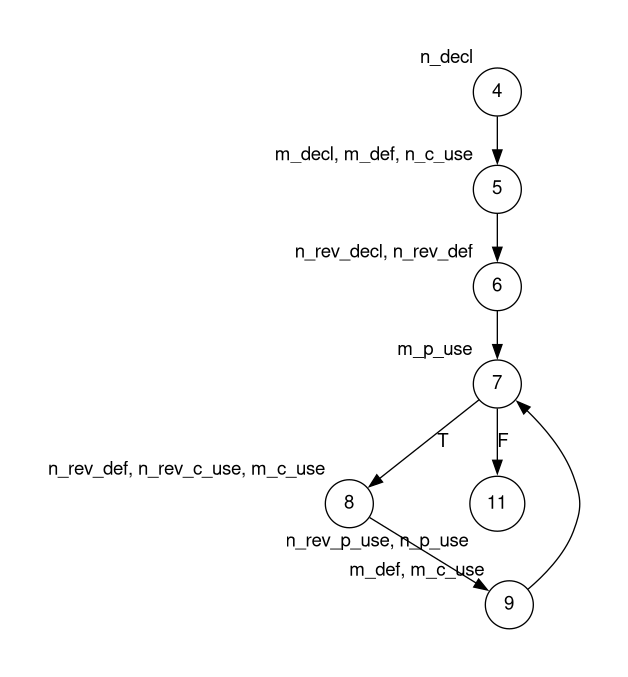
\includegraphics[scale=0.3]{palindrome_df_graph.png}
\end{figure}
\end{frame}

\begin{frame}


\frametitle{DU-Paths (n)}
\begin{itemize}
\item 5-11 
\end{itemize}
\end{frame}

\begin{frame}
\frametitle{DU-Paths (m)}
\begin{itemize}
\item 5-6-7 
\item 5-6-7-8-9
\item 9-7-8
\end{itemize}
\end{frame}

\begin{frame}
\frametitle{DU-Paths n\_rev}
\begin{itemize}
\item 6-7-8
\item 6-7-11
\item 8-9-7
\item 8-9-7-11
\end{itemize}
\end{frame}

\subsection{Test Suite}

\begin{frame}{Test Suite}
\begin{tabular}{c c}
Test      & \#1          \\
Test Path & 4-5-6-7-11          \\
Coverage  & 4-11, 5-6-7, 6-7-11          \\
Input     & n = 0 \\
Output    & true             
\end{tabular}

\noindent\makebox[\linewidth]{\rule{\paperwidth}{0.4pt}}

\begin{tabular}{c c}
Test      & \#2          \\
Test Path & 4-5-6-7-8-9-7-8-9-7-11          \\
Coverage  & 4-11, 5-6-7, 5-6-7-8-9, 8-9-7, 8-9-7-11, 9-7-8          \\
Input     & n = 11 \\
Output    & true
\end{tabular}
\end{frame}
\subsection{Comparison}
\begin{frame}{Comparison Data Flow vs. Branch coverage}
    For 100\% multiple-condition coverage, \(c = 1 \implies 2^c = 2\)
    \newline
    Matches exactly the number for covering all DU-paths. This doesn't have
    to be the case always. The last statement (returning the bool) is unusual
    as it doesn't change the branching of the program, but very much its behavior.
\end{frame}

\subsection{Practice}
\begin{frame}{Practice}
\center
But how does this actually look like? After all our Data Flow graphs are fortunately made for us humans and hence subjective!, but a compiler needs to be precise.
DU-paths (commonly known as Def-Use chains) are too complex to generate but go in the right direction.
The next step are Static Single-Assignment form (SSA) derived from the CFG.
\end{frame}

\begin{frame}[fragile]
    One can generate quiet helpful information that the compiler \(gcc \geq 4.0\) uses via
    \begin{verbatim}
        gcc palindrome.c -fdump-tree-all-graph
    \end{verbatim}
    Most importantly 
    \begin{verbatim}
        palindrome.c.cfg
    \end{verbatim}
    \begin{verbatim}
        palindrome.c.ssa
    \end{verbatim}
\end{frame}

\begin{frame}
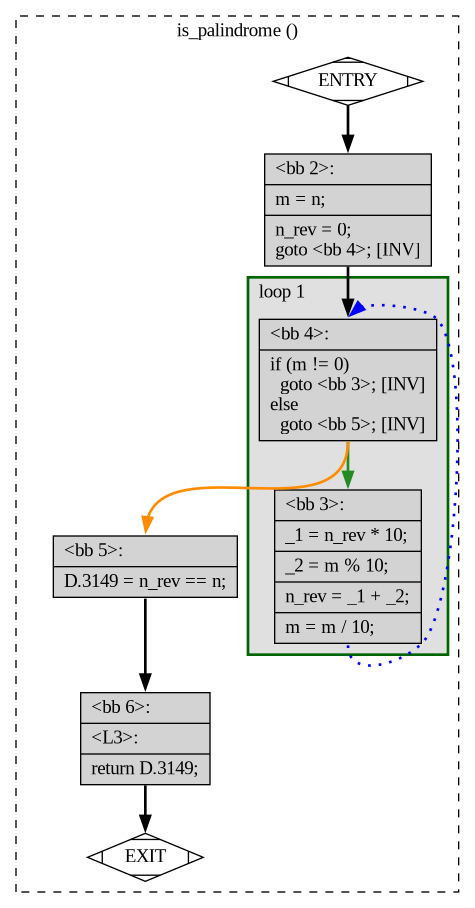
\includegraphics[scale=0.22]{palindrome_cfg.png}
\end{frame}


\begin{frame}
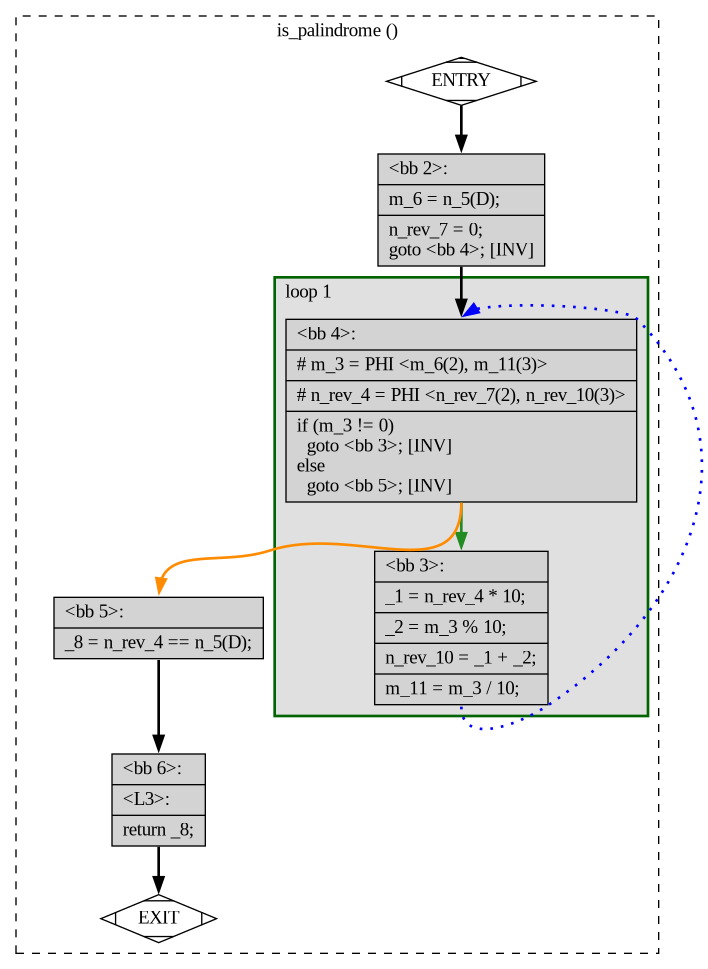
\includegraphics[scale=0.2]{palindrome_ssa.png}
\end{frame}

\begin{frame}[fragile]{Coverage}
\begin{tiny}
How about the statement/decision coverage? Really dependent on the languages ecosystem and most are happy with statement coverage.
For c there is gcov available. Running
\begin{verbatim}
#include <stdbool.h>
#include <assert.h>

bool is_palindrome(unsigned int n) {
    unsigned int m = n;
    unsigned int n_rev = 0;
    while (m > 0) {
        n_rev = (n_rev*10) + (m % 10);
        m = m / 10;
    }
    return n_rev == n;
}

int main() {
    assert(is_palindrome(0) == true);
    assert(is_palindrome(11) == true);
    return 0;
}
\end{verbatim}
\end{tiny}
\begin{verbatim}
$ gcc -Wall -fprofile-arcs -ftest-coverage palindrome_test.c
$ ./a.out
$ gcov -c palindrome_test.c
\end{verbatim}
\end{frame}

\begin{frame}[fragile]
\begin{tiny}
\begin{verbatim}
    File 'palindrome_test.c'
    Lines executed:100.00% of 11
    Branches executed:100.00% of 6
    Taken at least once:66.67% of 6
    Calls executed:50.00% of 4
    Creating 'palindrome_test.c.gcov'

    Lines executed:100.00% of 11
\end{verbatim}

\begin{verbatim}
    function is_palindrome called 2 returned 100% blocks executed 100%
            2:    4:bool is_palindrome(unsigned int n) {
            2:    5:    unsigned int m = n;
            2:    6:    unsigned int n_rev = 0;
            4:    7:    while (m > 0) {
    branch  0 taken 2
    branch  1 taken 2 (fallthrough)
            2:    8:        n_rev = (n_rev*10) + (m % 10);
            2:    9:        m = m / 10;
            -:   10:    }
            2:   11:    return n_rev == n;
            -:   12:}
            -:   13:
\end{verbatim}
\end{tiny}
\end{frame}

\subsection{Thanks}
\begin{frame}{The End}
    \center 
    Thank you for your attention!
\end{frame}

\end{document}
